\documentclass[12pt,a4paper]{article}
\usepackage[latin1]{inputenc}
\usepackage{amsmath}
\usepackage{amsfonts}
\usepackage{amssymb}
\usepackage{graphicx}
\usepackage{listings}
\usepackage{color}
\usepackage[margin=1in]{geometry}
\usepackage{caption}
\renewcommand{\theenumi}{\alph{enumi}}
\usepackage{minted}
\newcommand\tab[1][1cm]{\hspace*{#1}}

\lstset{ %
	frame=single,
	keywordstyle=\color{blue},
	numbers=left,
	numbersep=15pt,
	rulecolor=\color{black},
	framexleftmargin=8pt
}
\begin{document}
	\begin{titlepage}
		
		\newcommand{\HRule}{\rule{\linewidth}{0.5mm}} % Defines a new command for the horizontal lines, change thickness here
		
		\center % Center everything on the page
		
		%----------------------------------------------------------------------------------------
		%	HEADING SECTIONS
		%----------------------------------------------------------------------------------------
		
		\textsc{\LARGE Concordia University}\\[2.5cm] % Name of your university/college
		\textsc{\Large Project 2}\\[0.5cm] % Major heading such as course name
		\textsc{\large COMP 474}\\[0.5cm] % Minor heading such as course title
		
		%----------------------------------------------------------------------------------------
		%	TITLE SECTION
		%----------------------------------------------------------------------------------------
		
		\HRule \\[0.4cm]
		{ \huge \bfseries Network Suggested Items}\\[0.4cm] % Title of your document
		\HRule \\[1.5cm]
		
		%----------------------------------------------------------------------------------------
		%	AUTHOR SECTION
		%----------------------------------------------------------------------------------------
		
		\begin{minipage}{0.4\textwidth}
			\begin{flushleft} \large
				\emph{Authors:}\\
				Justin \textsc{Whatley} \\ 29472029 \\
				Mark \textsc{Chmilar} \\26827926
			\end{flushleft}
		\end{minipage}
		~
		\begin{minipage}{0.4\textwidth}
			\begin{flushright} \large
				\emph{Submitted to:} \\
				Dr. Houari \textsc{Smith} % Supervisor's Name
			\end{flushright}
		\end{minipage}\\[4cm]
		
		% If you don't want a supervisor, uncomment the two lines below and remove the section above
		%\Large \emph{Author:}\\
		%John \textsc{Smith}\\[3cm] % Your name
		
		%----------------------------------------------------------------------------------------
		%	DATE SECTION
		%----------------------------------------------------------------------------------------
		
		{\large \today}\\[4cm] % Date, change the \today to a set date if you want to be precise
		
		%----------------------------------------------------------------------------------------
		%	ENCS certification
		%----------------------------------------------------------------------------------------
	
		We certify that this submission is the original work of members of the group and meets the Faculty's Expectations of Originality
		
		%----------------------------------------------------------------------------------------
		
		\vfill % Fill the rest of the page with whitespace
		
	\end{titlepage}
	
	
	\subsection*{Intelligent System}
		An expert system would provide sufficient means to address the computational aspects of the problem, given simple logic to determine suggested item, but could not be properly integrated into the Amazon environment. A knowledge based system could be used if we wanted adaptive learning responses from network selections. For instance, if you repeatedly followed links from certain individuals in your network, a knowledge base system (KB) could adapt from this information and provide you more feedback from the peers with which you share more purchasing interests. Although this offers one possible solution, it is assumed that network information is already predetermined by Amazon and, thus, such learning procedure would be require unnecessary extra work and computational overhead. 
		\\\\
		Consequently, we will use a simple embedded agent that interacts autonomously with the Amazon server environment. This will primarily be a reactive agent, without learning capabilities. The reason for avoiding learning and adaptivity for the agent is the complexity of having a learning and adaptive agent would be too expensive to justify its implementation - particularly in this case where Amazon has Personal Network data with which to weigh decisions. Although a multi-agent system would also be possible for this intelligent system, we believe there are too few interacting components to justify this form of implementation. This last decision is based on the assumption that everything we need to develop a suggested item based on a peer-purchase can be obtained directly from the peer network. 
		\\\\
	\subsection*{Knowledge Representation}
		The knowledge representation will be encoded into database tables. For efficiency, the data will be encoded into Amazon's native NoSQL database which will be able to execute queries much more quickly. 
		\\\\
		The following includes the general structure and domain constraints placed on the data. Data validation will ensure valid insertions to the knowledge base and data structures mentioned describe encoding while in server memory: 
		\\\\
		\textbf{Network types:} limited to the strings "TN", "KN", or "VN". \\
		\\
		\textbf{Customers:} a hash map that has customer-ids as keys\\
		\\
		\textbf{Customer-id:} a hash map that allows keys: "network" and "purchased-items"\\
		\\
		\textbf{Network:} a hash map that has the following keys: "tn", "kn", and "vn"\\
		\\
		\textbf{TN:} an int array representing other customer id num.\ in Top Network (must be positive).\\ 
		\\
		\textbf{KN:} an int array representing other customer id num.\ in Key Network (must be positive). \\
		\\
		\textbf{VN:} an int array representing other customer id num.\ in Vital Network (must be positive).\\ 
		\\
		\textbf{Purchased-items:} an array that allows elements which are objects representing a customer's purchase.\\
		\\
		\textbf{Customer person object:} a hash map with the keys: "date" and "product"\\
		\\
		\textbf{Date:} a string representing the date of purchase, in the format yyyy-mm-dd, eg: "2017-04-31"\\
		\\
		\textbf{Product:} a hash map with the following keys: "name", "product-id", "categories", "rating", "price"\\
		\\
		\textbf{Name:}  a string representing the name of the purchased item \\
		\\
		\textbf{Product-id:} a positive integer representing the product id of the 
		purchased item\\
		\\
		\textbf{Categories:} an array of strings, where each element is a item category that the purchased item falls under. There is no limit on the number of categories in the array\\
		\\
		\textbf{Rating:} a decimal number (with one decimal place) between 0.0 and 5.0\\
		\\
		\textbf{Price:} a positive decimal number (with two decimal places)\\
		\\\\
		This JSON object serves as an outline for the organization of the data. This design is a proof of concept and will be replaced by Amazon's native NoSQL database later.  \\
		
		For example (insert JSON here):
		\inputminted{json}{knowledge-representation.json}
		
	\subsection*{Reasoning}
		Automated reasoning will be used to determine what purchased-items to display from your network. The approach will use Bayesian reasoning through a Bayesian Network. 
		\\\\
		The Bayesian Network will allow us to establish a criteria by which to decide when to include items purchased by peers in order to maximize sales. This reasoning will be important, as arbitrarily assigning items purchased by peers as suggested for you would do little to improve sales. 
		\\\\
		Initially, we will consider certain network-precedence, time passed since last purchase and peer-rating: 
		\\\\
		\textbf{Network-precedence:} The Personal Network level, TN, KN, and VN, will be used to weigh the value of an item purchased by the peer for the user. This preference will be exponential, where the user TN will be worth considerably more than the KN, which, in turn, will be worth considerably more than the VN (e.g., weights could be TN = 1, KN = 0.4, VN = 0.1). The network-preference value will ensure that only the most pertinent items are presented, by increasing the likelihood that proximity to the user is factored into item suggestions. 
		\\\\
		\textbf{Time passed since last purchase:} Here the amount of time passed will negatively impact the likelihood the item will be suggested. That is, given trending popularity, an item was purchased two-years ago is less likely to be relevant to the user than if the item was purchased recently. Further, recently purchased items are more likely to promote peer-review of items and discussion about the Amazon platform, as the user may ask the person in their network whether they enjoyed they will recommend the item. 
		\\\\
		\textbf{Peer-Rating:} The peer-rating will increase the likelihood that such an item will be displayed to the user. The rating will act synergistically with the Personal Network level. Given a high-rating by a peer that is close to the user, the item is very likely to be recommended. Conversely, a low-rating by the peer who is close to the user will decrease the likelihood that the item will be recommended for the user. In order to optimize suggestions, negative-ratings will counteract positive-ratings from other peers. Further, a low-rating by high level networks will carry more weight than a positive rating on a low level network - ensuring that such an item will not be displayed. 
		\\\\
		As the system evolves and and demonstrates its utility, we will fine-tune the process and adjust criteria in order to maximize sales. 
		\\\\
		Sample Bayesian Network:
		\begin{center}
			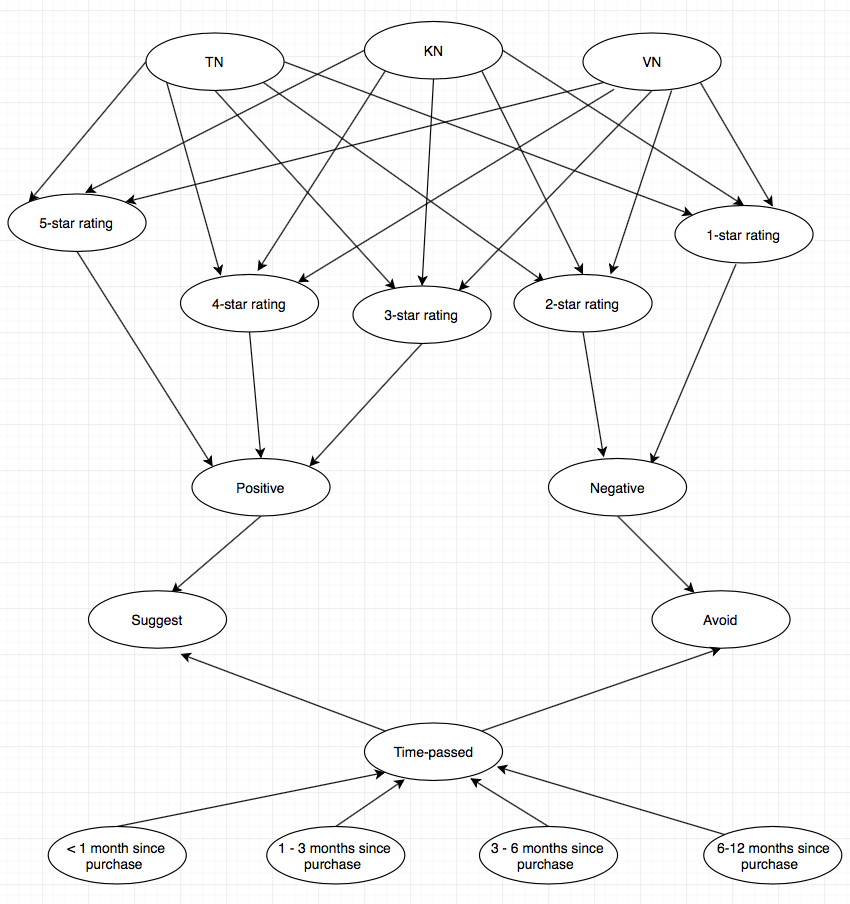
\includegraphics[width=1\linewidth]{bayes}
		\end{center}
		
		Probability tables are used in this case to capture the likelihood that an item should be suggested or avoided. From this, we can get aggregate "Suggest" and "Avoid" results by iterating through the user's Personal Network to see how individual items rank - Avoid rankings will detract from Suggest rankings.  
		\\\\
		The values in the tables will be established initially by assessing purchase history within the network to weigh the importance of each node. Subsequent analysis of the system will serve to fine-tune the probabilities to maximize sales. However, the tables data should fit the following guidelines: The closer network association the higher the value of ratings. Ratings from 3 to 5 hold increasing importance with respect to Positive rankings, while ratings from 2 to 1 hold increasing importance with respect to Negative rankings.  Time passed will determine relevance of suggestion or opposition to the purchase suggestion.
		\\\\
	\subsection*{Programming Language}
		Prolog is Turing complete and, thus, can be used to solve this problem. Thus, it would be possible to prototype the system using Prolog, but far from ideal. Prolog is an effective language to facilitate implementation is when you have a known goal and intermediary steps for which the logic is difficult to define. When the intermediary steps are difficult, Prolog will make development easier by letting the compiler handle the logic required to attain the goal. 
		\\\\
		For example:
\begin{minted}{prolog}
% Facts
bought(user1, item1).
bought(user2, item1).
bought(user3, item2).

% Sample Rule - if at least two people in network purchased an item
two_purchased(user1, ITEM) :- 
bought(CLIENT, ITEM), bought(CLIENT, ITEM), X = ITEM.
\end{minted}
		For this agent system like we have, however, the intermediary steps are simple to define and the goal is more complex. We are trying to generate a new suggested items based on the available personal-network data - with operations that should be flexible without a clearly defined goal. Because Amazon wants to create this quickly, we will use the Python programming language. This language is intuitive and is often used for rapid deployment. Based on the impact of the network item-suggestion program, later optimizations could use more rigorous languages to improve performance (e.g., Java, Go, C++).
		
		
		\subsection*{Components and System Structure}
		
		
		
		
		
		\subsection*{Development Methodology}
		
		The methodology we will use to in order to develop the program is Agile. This is a common software engineering process that allows developers to quickly develop software through an iterative process that takes into account mistakes and feedback in order to adjust course. This methodology is the best approach because it will ensure that Amazon will have the system up and running with the least possible delay. 
		\\\\
		The Agile development will include a planning phase for a two-week sprint, where developers will attempt to complete the tasks defined in the planning phase. A quick progress report will be given orally every morning at a 15 minute scrum, in order to keep everyone informed, get input from peers or re-allocate developer resources in the case where developer is blocking on some issue. This approach will help define milestones, assess progress, and re-conceptualize what needs to be done, if necessary. Consequently, this approach will help us implement the agent system, test it and make any necessary changes, while accommodate a more flexible development process. 
		
\end{document}